%%%%%%%%%%%%%%%%%%%%%%%%%%%%%%%%%%%%%%%%%%%%%%%%%%%%%%%%%%%%%%%%%%%%%%%%%%%%%%%%%%%%%%%%%%%%%
%%									Chapitre 3												%
%%%%%%%%%%%%%%%%%%%%%%%%%%%%%%%%%%%%%%%%%%%%%%%%%%%%%%%%%%%%%%%%%%%%%%%%%%%%%%%%%%%%%%%%%%%%%

\chapter{Vision événementielle et attention}
	\citationChap{
		On ne voit que ce que l'on regarde.
	}{Maurice Merleau-Ponty}
	\minitoc
	\newpage

%%%%%%%%%%%%%%%%%%%%%%%%%%%%%%%%%%%%%%%%%%%%%%%%%%%%%%%%%%%%%%%%%%%%%%%%%%%%%%%%%%%%%%%%%%%%%



% Début du chapitre			
	\section{Introduction}

	Ce chapitre regroupe les travaux que nous avons effectués sur l'utilisation de caméras évènementielles, expliquées dans le prochain paragraphe, en combinaison avec des champs neuronaux dynamiques (DNF) que nous avons présenté dans le premier chapitre. Nous présenterons les différents mécanismes que nous avons développés et mis en œuvre jusqu'à notre système attentionnel. Celui-ci combine les modèles présentés dans ce chapitre et la détection de nouveauté du chapitre 2. L'objectif étant  d'augmenter le niveau d'abstraction de notre modèle et de rendre une application dans un système embarqué la plus efficiente possible.

	A la différence des caméras classiques qui acquièrent des images à une certaine cadence proche de la milliseconde, les capteurs évènementiels détectent au niveau des pixels tout changement de luminosité de façon asynchrone à une résolution temporelle avoisinant la microseconde. L'information transmise n'est pas une image, mais uniquement des évènements asynchrones qui contiennent la position du pixel, l'horodatage et la polarité du changement (+1 si la luminosité augmente; -1 si elle diminue). Les DNF que nous avons utilisé ayant eux un taux de rafraîchissement fixe, nous avons intégré ces évènements sur ce pas de temps et produit une image de tous les changements qu'il y a eu dans cet intervalle. C'est un capteur qui est plus proche conceptuellement de la perception humaine que les caméras classiques. Il a aussi l'avantage d'avoir une très grande plage dynamique et possède un temps de latence très faible. \cite{gallego2019event}

	Il n'existe pas à notre connaissance de base de données disponible combinant à la fois des évènements et des images classiques correspondantes. Il est possible de recréer des évènements d'après des images \cite{hu2021v2e}, mais cela reste un résultat simulé, et nous avions à notre disposition une caméra évènementielle. Nous avons donc combiné cette caméra évènementielle avec une caméra classique en les synchronisant logiciellement pour obtenir les deux modalités en une fois. Les sections suivantes utilisent des images et évènements provenant de ces captures, ce qui nous permet de combiner la détection de nouveauté sur des images standard avec des DNFs sur des évènements.

	\newpage

	\section{Détection de mouvements}

	Le rôle de la première couche pour traiter les événements de la caméra sera de transformer les informations ponctuelles dans le temps et l'espace qu'envoie la caméra en zones de mouvements continues, facilitant le travail des couches supérieures. Pour ce faire, nous utiliserons des DNF, particulièrement appropriés par leur capacité d'intégration de l'information, et de leur robustesse au bruit très présent dans ce type de caméra. Habituellement, on utilise des DNF à deux dimensions pour gérer des images. Cependant cela représente 307 200 neurones avec notre caméra 640$\times$480, tous connectés dépendants les uns des autres, et devant être recalculés à chaque itération. Nous souhaitons que la première couche soit simple et rapide, alors nous avons choisi d'utiliser deux DNF à une dimension, un pour chaque axe.

	\begin{figureth}
		\begin{subfigureth}{\textwidth}
			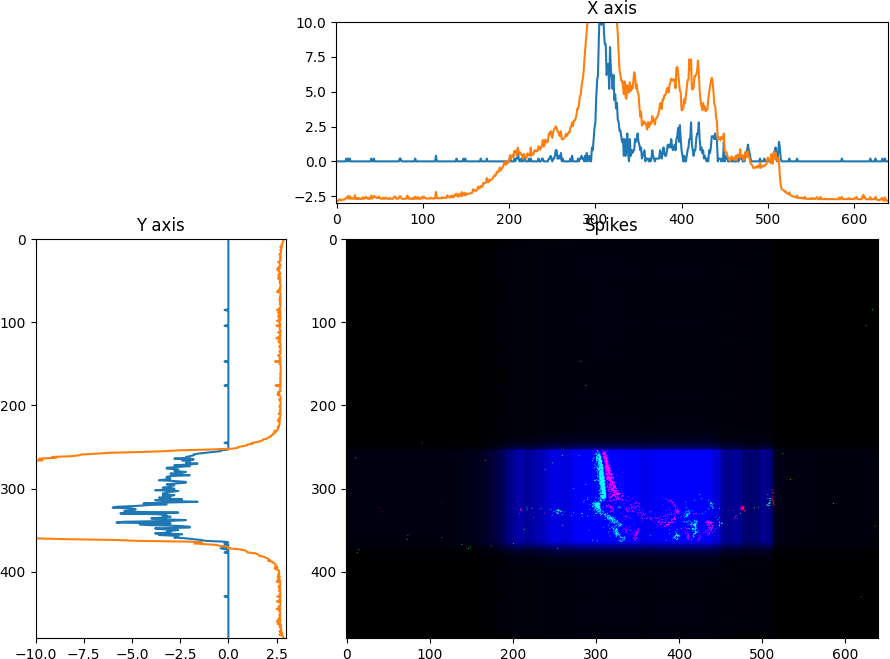
\includegraphics[width=\linewidth]{tracking/plane}
		\end{subfigureth}
		\caption[Détection de mouvements avec DNF sur caméra événementielle]{Détection de mouvements avec DNF sur caméra événementielle. Les points verts et rouges dans l'image correspondent respectivement aux augmentations et réductions de luminosités détectés par la caméra. La somme des événements de chaque axe est affichée dans les courbes bleues qui sont en entrée des deux DNF. En orange sont les potentiels des DNF. On calcule le produit dyadique de la sortie des DNF, c'est à dire après la sigmoïde, pour obtenir la zone de détection de mouvement en bleu sur l'image.}\label{fig:track:plane}
	\end{figureth}

	Les DNF peuvent fonctionner à la fois en mode impulsionnel et en mode discrétisé. Nous avons choisi le second mode, car il est plus rapide à calculer et plus stable. Sa vitesse ne dépend pas du nombre d'événements à traiter, contrairement au modèle impulsionnel. Il nous a donc fallu intégrer les évènements avec un pas de temps que nous avons mis à 10 ms. Il est aussi possible de le placer à 1 ms ou en dessous, si l'on souhaite détecter des mouvements très rapides. Il y aura juste plus de mises à jour par seconde des potentiels du DNF, et donc plus de calculs. Nous n'avons pas utilisé la polarité des évènements, uniquement si un pixel détectait un changement ou pas.

	Les événements que nous recevons de la caméras sont très bruités. Il existe notamment certains pixels défectueux qui envoient en permanence des événements. Il s'agit de bruit artificiel dû à la technologie et non présent dans la nature. Il n'est donc pas particulièrement intéressant pour nous de l'inclure dans notre étude. Nous avons donc désactivé logiciellement ces pixels défectueux. Le bruit présent dans la nature et plus diffus, a lui été conservé. Le résultat est présenté sur la figure \ref{fig:track:plane}.

	\subsection{Multi cibles}

	\begin{figureth}
		\begin{subfigureth}{\textwidth}
			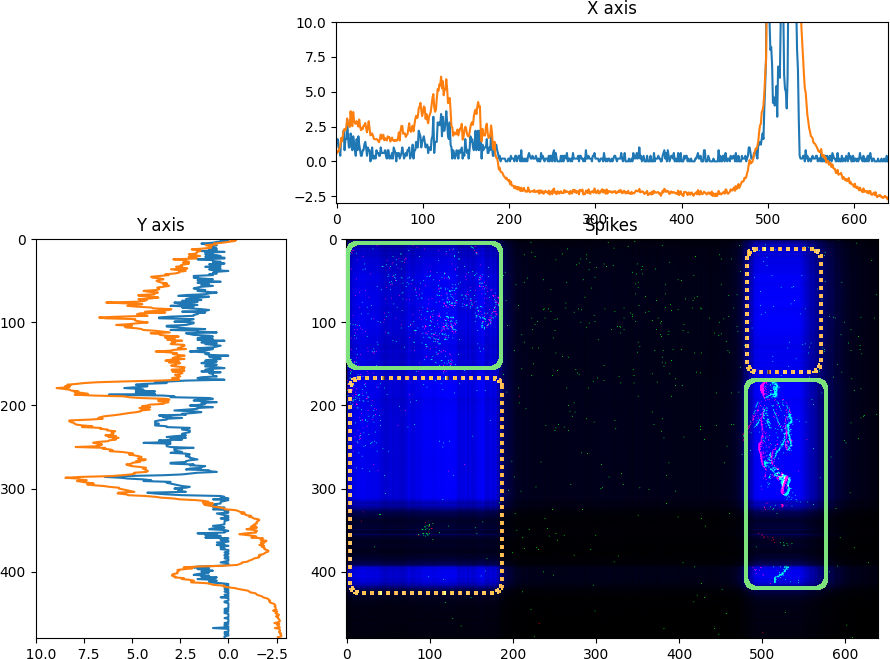
\includegraphics[width=\linewidth]{tracking/walk_with_contours}
		\end{subfigureth}
		\caption[Détection de mouvements multicible avec DNF sur caméra événementielle]{Détection multicible. Il y a deux stimulus dans la scène, entourés par des lignes vertes. La personne qui se déplace en bas à droite et un mouvement dans un arbre en haut à gauche. Les activations parasites, dû à la projection de deux détections en 1D vers du 2D sont entourés par des pointillés orange.}\label{fig:track:multi}
	\end{figureth}

	Notre système est également capable de suivre de multiples cibles, mais au prix de détections parasites. En effet, passer de 2 dimensions à 2 fois 1 dimension pour ensuite projeter à nouveau en 2 dimensions est efficace en calculs, mais il y a une perte d'informations dans le processus. Lorsque l'on passe en 1 dimensions, on ne connaît que les valeurs sur chaque axe des deux stimulus, sans pouvoir les associer entre elles. Un exemple est présenté sur la figure \ref{fig:track:multi}.

	\subsection{Paramètres}

	Le paramétrage de DNF est une tâche délicate. Nous avons ajusté à la main les valeurs de chaque paramètre à l'aide de nos connaissances sur ces modèles. Bien que nous n'ayons pas beaucoup modifiés les paramètres entre les deux exemples que nous avons présentés, il est possible qu'une séquence nouvelle ne fonctionne pas avec les paramètres que nous avons sélectionnés, et qu'il faille reparamétrer les DNF pour que cela fonctionne comme attendu. Les deux DNF de chaque axe utilisent les mêmes paramètres. Chaque événement compte pour 0.2 dans l'entrée des DNF pour une meilleure visualisation sur les figures, car mettre cette valeur à 1 et diviser le gain par 5 aurait eu le même effet sur le DNF.


	\begin{tableth}
	\label{tab:recap:param}
	\caption[Paramètres DNF 1D]{Paramètres DNF 1D}
	\begin{tabular}{|c|cc|}
		\hline
		Paramètre & Figure \ref{fig:track:plane} & Figure \ref{fig:track:multi}\\
		\hline
		$\delta$t & 0.01 & 0.01\\
		$\tau$ & 0.05 & 0.05\\
		Coef. excitateur & 4.5 & 4.5\\
		$\sigma$ excitateur & 0.01 & 0.01\\
		Gain & 4 & 1.5\\
		Repos $h$ & -3 & -3\\
		\hline
	\end{tabular}
	\end{tableth}

	\newpage

	\section{Combinaison avec la détection de nouveauté}

	La détection de mouvement présentée dans la section précédente a des points communs avec la détection de nouveauté de la SOM. En effet, chaque cible détectée par la détection de nouveauté sera nécessairement également détectée par la détection de mouvement. Car la nouveauté ne peut apparaître qu'avec du mouvement. L'inverse n'est cependant pas vrai (il peut y avoir du mouvement sans nouveauté), et ce principe ne compte que lors de l'apparition de nouveauté. Si de la nouveauté s'arrête de se déplacer, elle n'apparaîtra plus comme mouvement, mais sera toujours de la nouveauté.

	La détection de mouvement étant beaucoup plus rapide que la détection de nouveauté, nous pouvons utiliser celle-ci comme déclencheur de la détection de nouveauté dans une zone particulière de l'image. Ainsi, la détection de nouveauté ne sera appelée que lorsque du mouvement apparaîtra dans l'image, et limitera le calcul de la SOM à une zone d'intérêt dans l'image. Un exemple est montré sur la figure \ref{fig:opti:spike}.

	\begin{figureth}
		\begin{subfigureth}{\textwidth}
			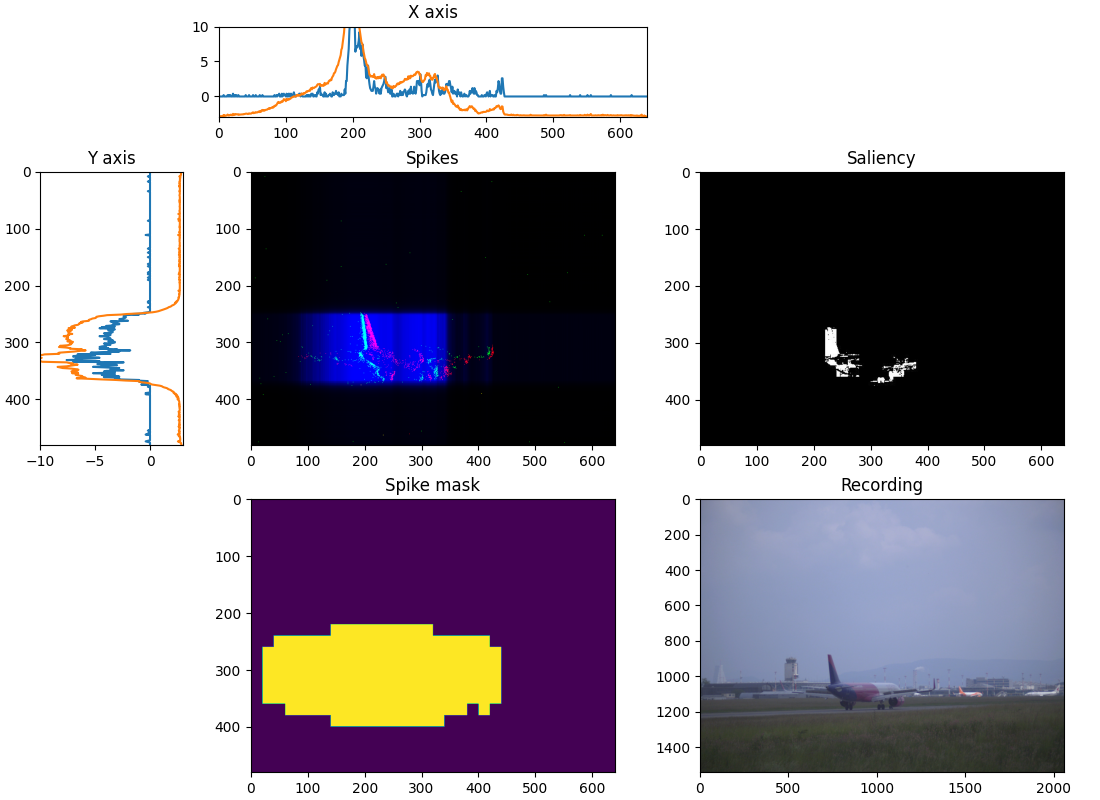
\includegraphics[width=\linewidth]{tracking/spike_opti}
		\end{subfigureth}
		\caption[Combinaison SOM et DNF par zone d'intérêt]{Un exemple de combinaison possible entre une caméra évènementielle et la détection de nouveauté avec une SOM. Les DNF travaillant sur les entrées évènementielles permettent la création d'une zone d'intérêt (image en bas à gauche). Cette zone d'intérêt sert à concentrer les efforts de la SOM là où de la nouveauté a des chances d'apparaître.}\label{fig:opti:spike}
	\end{figureth}

	Le masque est obtenu en appliquant un seuil sur la combinaison des deux DNF par le produit dyadique. La valeur du seuil a été choisie pour englober la zone d'intérêt le plus possible sans dépasser au delà. Un seuil trop bas a pour conséquence qu'une activation d'un seul DNF suffira à dépasser le seuil, et ainsi la zone d'intérêt formera une "croix" avec pour centre la vraie zone d'intérêt. Un bon seuil est donc juste assez haut pour éviter la croix, mais le plus bas possible pour ne rien perdre dans la zone d'intérêt.

	\begin{tableth}
	\caption[Gains grâce à la combinaison SOM-DNF]{Estimation de gains potentiels avec cette combinaison de SOM-DNF. Il n'y a pas beaucoup de nouveauté qui est perdue (83\% de la sortie de la SOM conservée au minimum), et les pertes sont en majorité du bruit. Les gains quand à eux peuvent aller de 2 fois plus rapide à 10 fois, en fonction de la taille du signal, et du bruit ambiant.}
	\begin{tabular}{|c|c|c|}
		\hline
		Séquence & Taux de positifs conservés & Taux d'imagettes évaluées\\
		\hline
		Plane & 98,9\% & 10\% \\
		Walk & 83,6\% & 43\% \\
		Highway & 90,8\% & 18,3\% \\
		\hline
	\end{tabular}
	\label{tab:nbr:optidnf}
	\end{tableth}

	Le tableau \ref{tab:nbr:optidnf} présente quelques métriques pour estimer les gains potentiels de cette méthode sur des séquences que nous avons enregistrées. Les gains dépendent fortement de la taille des objets en mouvements (plus ils sont gros, plus la SOM sera sollicitée), et du bruit ambiant. En effet, des mouvements sans nouveauté dans le fond d'une image solliciterons la SOM pour les classer en nouveauté ou non continuellement. Mais si il n'y a pas de signal et que les DNF ne s'activent pas à cause du bruit, la SOM peut être complètement ignorée et la caméra non évènementielle éteinte. Cela permet donc un mode d'observation passif consommant peu d'énergie (uniquement avec caméra évènementielle et DNF), qui peut automatiquement devenir actif en fonction de la scène observée.

	\newpage

	\section{Mécanisme attentionnel}

	Cette section présentera notre tentative de former un mécanisme attentionnel avec un DNF en combinant la détection de nouveauté par images et la détection de mouvement par évènements. Notre attention aura pour objectif de se focaliser sur un unique stimulus à la fois dans la scène. Il devra également pouvoir suivre en continu la cible sélectionnée dans le champ visuel.

	\subsection{DNF pour l'attention}

	Des modèles attentionnels ont déjà été employés pour effectuer de l'attention à partir d'entrée évènementielles directement \cite{evanusa2019event}. Nous souhaitons plutôt placer notre attention au niveau d'abstraction le plus élevé de notre modèle, c'est à dire après la détection de mouvement des DNF et la détection de nouveauté de la SOM.

	Pour produire l'attention, nous avons cette fois-ci choisi d'utiliser un DNF à deux dimensions. En effet utiliser deux DNF à une dimension dans ce cas pourrait amener des problèmes de localisation spatiales. Si il y a plusieurs cibles dans la scène visuelle, il est possible que les deux DNF ne sélectionnent pas la même. Par exemple si il y en a une étalée horizontalement et une autre étalée verticalement et toutes les deux ont une aire similaire, le DNF de l'axe $x$ se focalisera préférentiellement sur la cible verticale et le DNF de l'axe $y$ sur la cible horizontale, car les points seront plus denses lorsque projetés sur ces axes, et les neurones correspondants seront donc plus activés que ceux de l'autre cible et auront plus de chance de générer une bulle d'activité. Si les deux DNF ne produisent pas la bulle d'activité pour la même cible, alors il est possible que la combinaison des deux amène à être attentif à une zone vide de la scène.

	Utiliser un DNF à deux dimensions permet de ne pas avoir ce problème. Mais le nombre de neurones augmente en conséquence, et les coûts en calculs avec. Nous avons donc choisi de mettre un seul neurone pour couvrir une zone de 20 par 20 pixels. Pour notre entrée en 640 par 480, cela donne un DNF de 32 par 24 neurones, soit 768 neurones, le même ordre de grandeur que deux DNF à une dimension auraient donné. La perte de précision n'est pour nous pas un problème, car l'objectif ici n'est que de trouver une zone d'attention, pas d'entourer la forme de la nouveauté avec une grande précision. L'entrée de notre DNF consiste en une combinaison additive de la carte seuillée de la détection de nouveauté et du produit dyadique des deux DNF 1D de la détection de mouvement. Nous avons paramétré notre DNF de telle sorte qu'il faille un stimulus fort à la fois dans la détection de nouveauté et dans la détection de mouvement pour créer une bulle attentionnelle, et que celle-ci puisse se maintenir avec une seule des deux modalités. Si par exemple l'objet arrête de se déplacer et devient statique par exemple, alors la bulle attentionnelle restera fixée sur lui grâce à la détection de nouveauté uniquement.

	La paramétrisation d'un DNF pour la sélection est différente de la version multi-cibles des DNF 1D. Les paramètres sont montrés dans le tableau \ref{tab:recap:param2D}. Nous avons réduit la valeur de $\tau$ pour rendre le DNF plus réactif aux changements. Nous avons ajouté de l'inhibition pour permettre la formation d'une bulle de taille plus ou moins fixe autour du stimulus au centre de l'attention. Nous avons ajusté la valeur de l'excitation en conséquence. Le repos à été augmenté à -1 pour permettre à une bulle d'activité d'apparaître plus facilement, et nous avons mis de l'inhibition globale qui limite le DNF à l'apparition d'une seule bulle.

	\begin{tableth}
	\caption{Paramètres du DNF 2D attentionnel}
	\begin{tabular}{|c|c|}
		\hline
		Paramètre & Valeur\\
		\hline
		$\delta$t & 0.01 \\
		$\tau$ & 0.02 \\
		Coef. excitateur & 8 \\
		$\sigma$ excitateur & 0.01 \\
		Coef. inhibiteur & 5 \\
		$\sigma$ inhibiteur & 0.1 \\
		Gain & 1.5 \\
		Repos $h$ & -1 \\
		Inhibition globale $gi$ & 400 \\
		\hline
	\end{tabular}
	\label{tab:recap:param2D}
	\end{tableth}

	La figure \ref{fig:opti:attention} présente un exemple d'attention sur une séquence capturée au dessus d'une autoroute.

	\begin{figureth}
		\begin{subfigureth}{\textwidth}
			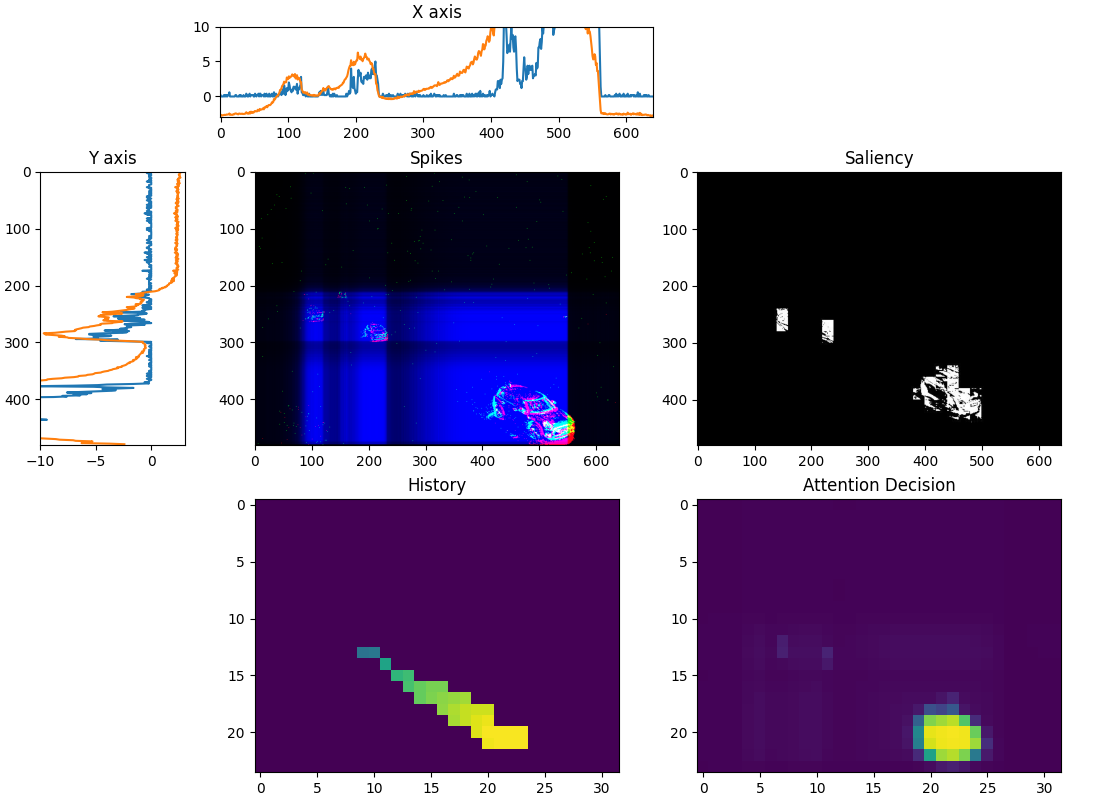
\includegraphics[width=\linewidth]{tracking/attention}
		\end{subfigureth}
		\caption[Exemple d'Attention avec DNF]{Un exemple d'attention avec un DNF. Le DNF attentionnel choisi parmi les 3 voitures dans l'entrée celle qui produit le plus de saillance, c'est à dire la plus visible dans la détection de nouveauté et qui produit le plus d'évènements. Ici, il s'agit de la voiture la plus proche. La zone d'attention est montrée dans la figure en bas à droite. Le suivi de la trajectoire, depuis la création de la bulle attentionnelle jusqu'à sa position actuelle est présentée dans la graphe en bas à gauche. On peut aussi remarquer que la détection de nouveauté et la caméra évènementielle placent la voiture à deux endroits légèrement différents. Cela est dû au fait que la caméra évènementielle est plus rapide et elle a détecté la progression du véhicule depuis la dernière image capturée par la caméra standard. Les données provenant de deux caméras différentes, les variations dans l'angle de vue et dans l'objectif amènent également à des différences dans la position des objets.}\label{fig:opti:attention}
	\end{figureth}

	\subsection{Séquence de détection}

	Avec notre modèle attentionnel actuel, nous pouvons organiser la dynamique d'un potentiel mécanisme de détection embarqué. La séquence de détection pourrait se dérouler de la façon suivante : 

	\begin{itemize}
		\item Le système est en "veille active". Seule la caméra évènementielle basse consommation est active, ainsi que la détection de mouvement par DNF.
		\item Une cible apparaît produisant un grand nombre d'évènements détectés par les DNF. Ils activent la caméra standard qui prend une photographie de son champ visuel. À partir de cette photo se fait la détection de nouveauté à l'endroit où se trouve la cible.
		\item Si pas de nouveauté n'est trouvée à cet endroit, alors l'attention ne s'active pas. La détection de mouvement continue de suivre la cible, et une détection de nouveauté est refaite à une faible fréquence.
		\item Si de la nouveauté a été trouvée, alors la combinaison de mouvement et nouveauté active le mécanisme attentionnel qui se focalise sur cette cible et suit et enregistre son déplacement. Une détection de nouveauté est faite à une fréquence rapide, et des mécanismes cognitifs plus avancés et coûteux en calculs peuvent être lancés sur la zone attentive.
		\item Lorsque l'objet disparaît, l'attention s'estompe également et le système retourne en "veille active".
	\end{itemize}

	Un tel fonctionnement dans un système embarqué permet des économies considérables en temps de calculs et en énergie et amène à une plus grande autonomie du système.

	\subsection{Évolutions possibles}

	Nous présenterons ici quelques pistes d'améliorations que l'on pourrait apporter à l'attention.

	\begin{itemize}
		\item La capacité de suivre plusieurs cibles. Cela peut-être fait en utilisant deux DNF attentionnel identiques, avec une connexion inhibitrice entre eux. Ainsi lorsque l'un d'eux choisi une cible. L'inhibition empêche l'autre DNF de choisir la même. Il se tournera donc vers la seconde cible la plus proéminente. Si il n'y en a pas, pas de bulle ne se formera. Utiliser deux mécanismes d'attention en simultané nous éloigne de l'inspiration biologique (les humains n'ont qu'une seule attention), mais cela peut-être utile pour certaines applications.
		\item L'attention peut être, comme chez l'homme, la base de processus cognitifs plus complexes. Dans notre exemple on pourrait imaginer un mécanisme capable d'identifier les voitures qui serait activé que sur les cibles sur lesquelles le système est attentif. Mais aussi des choses plus simples comme compter le nombre de voitures rouges empruntant cette autoroute. Le tout uniquement de façon neuromorphique.
		\item Une autre inspiration biologique serait d'ajouter une mémoire à court terme inhibitrice de l'attention. Cela permettrait d'effectuer une exploration séquentielle des différentes cibles présentes dans la scène, comme par exemple dans \cite{fix2011dynamic}.
	\end{itemize}
		
\bibliographystyle{francaissc}
\bibliography{Chapitre3/Biblio}